
% TODO : explain something
% canal blablabla
% probes : segment & points

see figure \ref{domain}
\begin{figure}[h!]
\centering
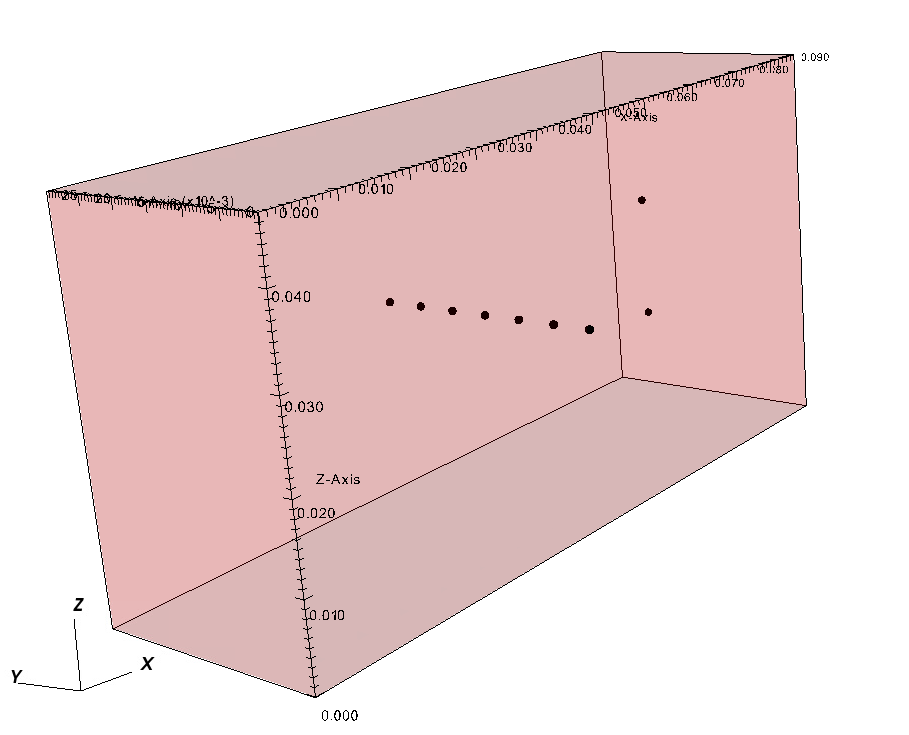
\includegraphics[width=.6\linewidth]{\orig/.tmp/../canal.png}
\caption{Description of the computational domain depicting the probes position.}
\label{domain}
\end{figure}



\section{Configuration}

This validation file was made to show what can be done with the Python post processing code. In this test case, we have 
three folders named sim\_1, sim\_2, sim\_3 with sim\_2 the continuation of sim\_1 and sim\_3 the continuation of sim\_2. 
The goal is to do statistical post processing of the results coming from the .son and .dt\_ev files. \\


\newpage
\section{Step time}
In this section, we will plot simulation step time. Other quantities can be displayed from .dt\_ev files
as long as the correct keyword is given.


\begin{figure}[h!]
\centering
\includegraphics[width=.6\linewidth]{\orig/.tmp/../sim_3/results/fig_1.png}
\caption{Evolution of step time.}
\label{fig1}
\end{figure}

\newpage
\section{Velocity}
Plots the instantaneous probes evolution of velocity field and fluctuations.


\begin{figure}[h!]
\centering  
\includegraphics[width=.6\linewidth]{\orig/.tmp/../sim_3/results/fig_2.png}
\caption{velocity}
\label{fig2}
\end{figure}


\begin{figure}[h!]
\centering
\includegraphics[width=.6\linewidth]{\orig/.tmp/../sim_3/results/fig_3.png}
\caption{Velocity fluctuation.}
\label{fig3}
\end{figure}


\newpage
\section{Density}
An example with an other field: the instantaneous density evolution. 


\begin{figure}[h!]
\centering
\includegraphics[width=.6\linewidth]{\orig/.tmp/../sim_3/results/fig_4.png}
\caption{Density instantaneous.}
\label{fig4}
\end{figure}



\newpage
\section{Pressure}
Displayong the pressure evolution, fluctuations and finally spatial mean over the segment.


\begin{figure}[h!]
\centering
\includegraphics[width=.6\linewidth]{\orig/.tmp/../sim_3/results/fig_5.png}
\caption{Pressure instantaneous.}
\label{fig5}
\end{figure}

\begin{figure}[h!]
\centering
\includegraphics[width=.6\linewidth]{\orig/.tmp/../sim_3/results/fig_6.png}
\caption{Spatial mean pressure.}
\label{fig6}
\end{figure}

\begin{figure}[h!]
\centering
\includegraphics[width=.6\linewidth]{\orig/.tmp/../sim_3/results/fig_7.png}
\caption{Spatial mean pressure.}
\label{fig7}
\end{figure}

\newpage

\section{Average windows on velocity}
Example of window averaging.

\begin{figure}[h!]
\centering
\includegraphics[width=.6\linewidth]{\orig/.tmp/../sim_3/results/fig_8.png}
\caption{Average windows.}
\label{fig8}
\end{figure}

\newpage

\section{Autocorrelation and Spectrum}
We can perform an autocorrelation of the velocity signal, the root of parabola fit gives us the taylor micro scale. 
After that, the energy spectrum is computed using welch method.

\begin{figure}[h!]
\centering
\includegraphics[width=.6\linewidth]{\orig/.tmp/../sim_3/results/fig_9.png}
\caption{Autocorrelation and parabola fit.}
\label{fig9}
\end{figure}

\begin{figure}[h!]
\centering
\includegraphics[width=.6\linewidth]{\orig/.tmp/../sim_3/results/fig_10.png}
\caption{Energy spectrum.}
\label{fig10}
\end{figure}


